\chapter{PDFs from reduced pseudo-ITD data:  \\ Pion Mass dependence for 170 ensemble}
Similarly to what done for the fine ensemble in Sec.~\ref{sec:discussion_sys},
the data for the ensemble 280 presented in Ref.~\cite{Joo:2020spy} can also be used to estimate pion mass effects
for results concerning the ensemble 170. The corresponding polynomial curves are plotted in Fig.~\ref{fig:sys_170}
as functions of the Ioffe-time.
\begin{figure}[h!]
    \centering
    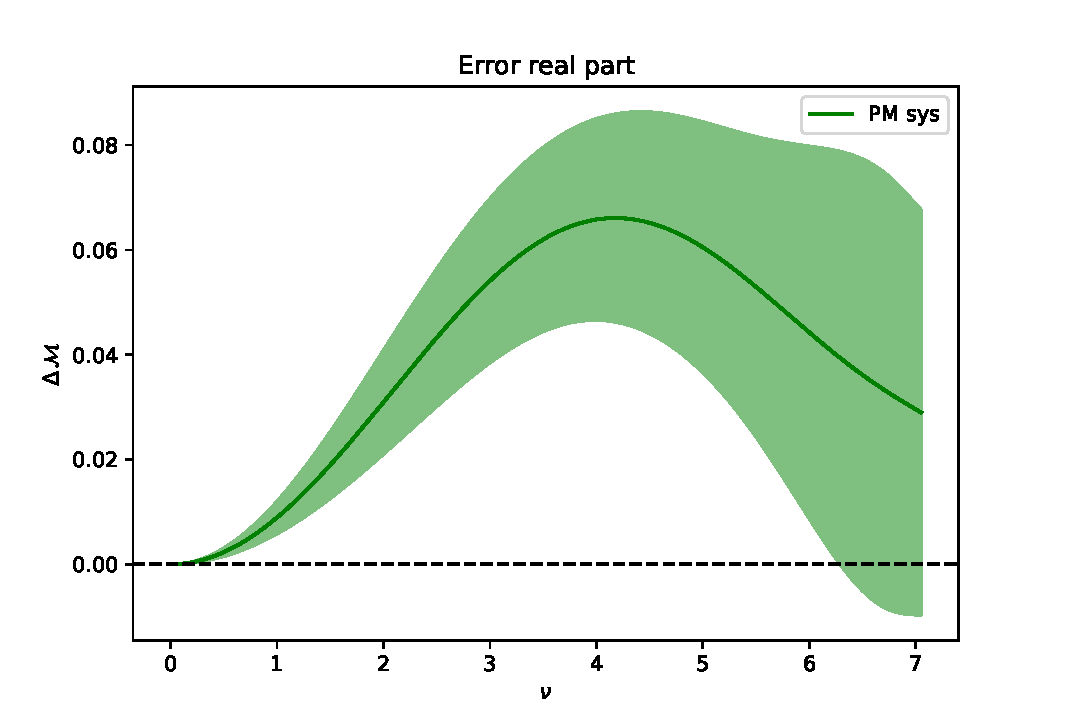
\includegraphics[width=0.49\linewidth]{real_sys_170.pdf}  
    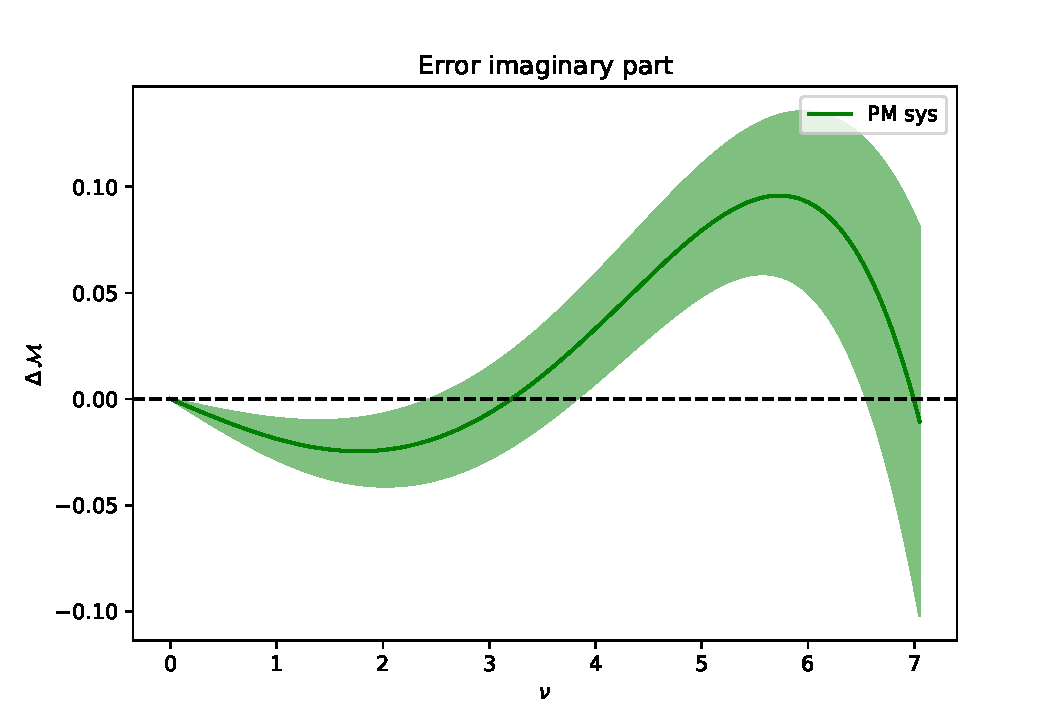
\includegraphics[width=0.49\linewidth]{imag_sys_170.pdf}
\caption{Pion mass (PM) systematic provided 
as functions of the ioffe-time $\nu$ for the real (left) and imaginary (right) part 
of the matrix element.}
\label{fig:sys_170}
\end{figure}

%
As in the case of the analysis for the fine ensemble, the curves in Fig.~\ref{fig:sys_170} are used 
to define a source of correlated systematic. The resulting PDFs, denoted as \textit{170-sys}, are 
plotted in Fig.~\ref{fig:res_170_sys} together with the results for the ensemble 170 presented in Sec.~\ref{sec:fit},
where only statistical uncertainties have been considered.
From Fig.~\ref{fig:res_170_sys} it is clear how introducing pion mass systematic effects in the analysis has very little impact on
the distributions, the major effect being a mild down shift of the central value of $V_3$ in the medium $x$ region.
\begin{figure}[h!]
    \centering
    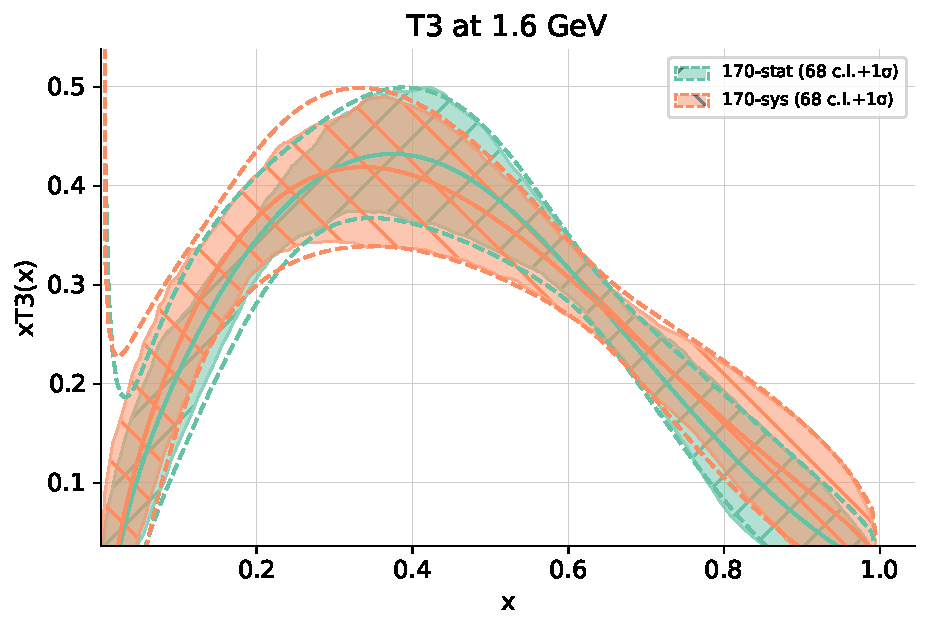
\includegraphics[width=0.49\linewidth]{T3_170_sys.pdf}  
    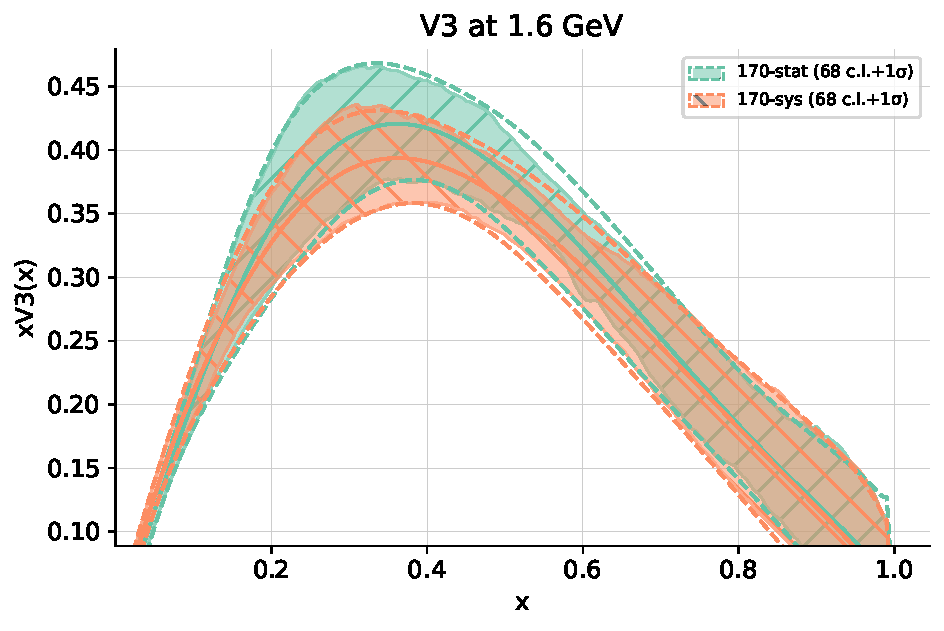
\includegraphics[width=0.49\linewidth]{V3_170_sys.pdf}
\caption{PDFs from the fits \textit{170-stat} and \textit{170-sys}.}
\label{fig:res_170_sys}
\end{figure}
We conclude that the mild pion mass dependence observed in pseudo-ITD data of Ref.~\cite{Joo:2020spy} has no sizable impact
on the final PDFs.
